\documentclass[aspectratio=169]{beamer}

%\usetheme{Pittsburgh}
\usetheme{metropolis}

\usepackage[utf8]{inputenc}

\usepackage{pgfplots}
\usepackage{pgfplotstable}
\usepackage{tikz}
\usepackage{xcolor}
\usetikzlibrary{automata, arrows.meta, shapes.geometric, positioning}

\usepackage{minted}
\usepackage{todonotes}
\usepackage[normalem]{ulem}
\usepackage[export]{adjustbox}



% \newtheorem{theorem}{Theorem}[chapter]
% \newtheorem{corollary}{Corollary}[theorem]
% \newtheorem{lemma}[theorem]{Lemma}
% \newtheorem{proposition}[theorem]{Proposition}
% \theoremstyle{definition}
% \newtheorem{example}[theorem]{Example}
% \newtheorem{definition}[theorem]{Definition}



\newcommand{\ZZ}{\mathbb{Z} \times \mathbb{Z}}
\newcommand{\nequiv}{\not\equiv}
\newcommand{\nequivp}{\nequiv_{\Psi,\T}}
\newcommand{\equivp}{\equiv_{\Psi,\T}}
% \renewcommand{\labelenumii}{\arabic{enumii}.}
\newcommand{\join}{\sqcup}
\newcommand{\meet}{\sqcap}
\newcommand{\widen}{\nabla}
\newcommand{\narrow}{\Delta}
\newcommand{\sem}[1]{\llbracket#1\rrbracket}
\newcommand{\Z}{\mathbb{Z}}
\renewcommand{\L}{\mathcal{L}}
\newcommand{\T}{\mathcal{T}}
\newcommand{\Set}{\mathcal{S}}
\newcommand{\oT}{{\overline{\mathcal{T}}}}
\newcommand{\F}{\mathcal{F}}
\newcommand{\A}{\mathcal{A}}
\newcommand{\X}{\mathcal{X}}
\newcommand{\V}{\mathcal{V}}
\newcommand{\malloc}{\textsf{malloc}}
\newcommand{\nf}{\textsf{nf}}
\newcommand{\restr}[2]{\left.\kern-\nulldelimiterspace#1\vphantom{|}\right|_{#2}}
\newcommand{\otau}{\overline{\tau}}
\newcommand{\angl}[1]{\langle#1\rangle}
% \newcommand{\widen}{\mathop{{\sqcup}\hspace*{-0.6em}\raisebox{.4ex}{\setlength{\unitlength}{1em}\line(1,0){.53}}}}
% \newcommand{\narrow}{\mathop{{\sqcap}\hspace*{-0.6em}\raisebox{.9ex}{\setlength{\unitlength}{1em}\line(1,0){.50}}}}
\newcommand{\ignore}[1]{}
\newcommand{\cpo}{\textsf{C-2PO}}
\newcommand{\goblint}{\textsc{Goblint}}
\newcommand{\find}[1]{\textsf{find}(#1)}
\newcommand{\union}[3]{\textsf{union}(#1, #2, #3)}
\newcommand{\closure}[4]{\textsf{closure}(#4, #1 = #2 + #3)}
\newcommand{\ext}[2]{\textsf{ext}\,{#1}\,{#2}}
\newcommand{\enter}{\textsf{enter}}
\newcommand{\combine}{\textsf{combine}}
\newcommand{\base}{\emph{base}}
\newcommand{\vareq}{\emph{var\_eq}}
\newcommand{\cpou}{$c$-$2po_1$}
\newcommand{\cpod}{$c$-$2po_2$}
\newcommand{\cpot}{$c$-$2po_3$}
\newcommand{\cpoq}{$c$-$2po_4$}


% Define TUM corporate design colors
% Taken from http://portal.mytum.de/corporatedesign/index_print/vorlagen/index_farben
\definecolor{TUMBlue}{HTML}{0065BD}
\definecolor{TUMSecondaryBlue}{HTML}{005293}
\definecolor{TUMSecondaryBlue2}{HTML}{003359}
\definecolor{TUMBlack}{HTML}{000000}
\definecolor{TUMWhite}{HTML}{FFFFFF}
\definecolor{TUMDarkGray}{HTML}{333333}
\definecolor{TUMGray}{HTML}{808080}
\definecolor{TUMLightGray}{HTML}{CCCCC6}
\definecolor{TUMAccentGray}{HTML}{DAD7CB}
\definecolor{TUMAccentOrange}{HTML}{E37222}
\definecolor{TUMAccentGreen}{HTML}{A2AD00}
\definecolor{TUMAccentLightBlue}{HTML}{98C6EA}
\definecolor{TUMAccentBlue}{HTML}{64A0C8}



\title[\cpo{}: A Weakly-Relational Pointer Analysis]{\cpo{}: A Weakly-Relational Pointer Analysis for Goblint}
\author{Rebecca Ghidini}
\date{19. September 2024}
\titlegraphic{\raggedleft\vfill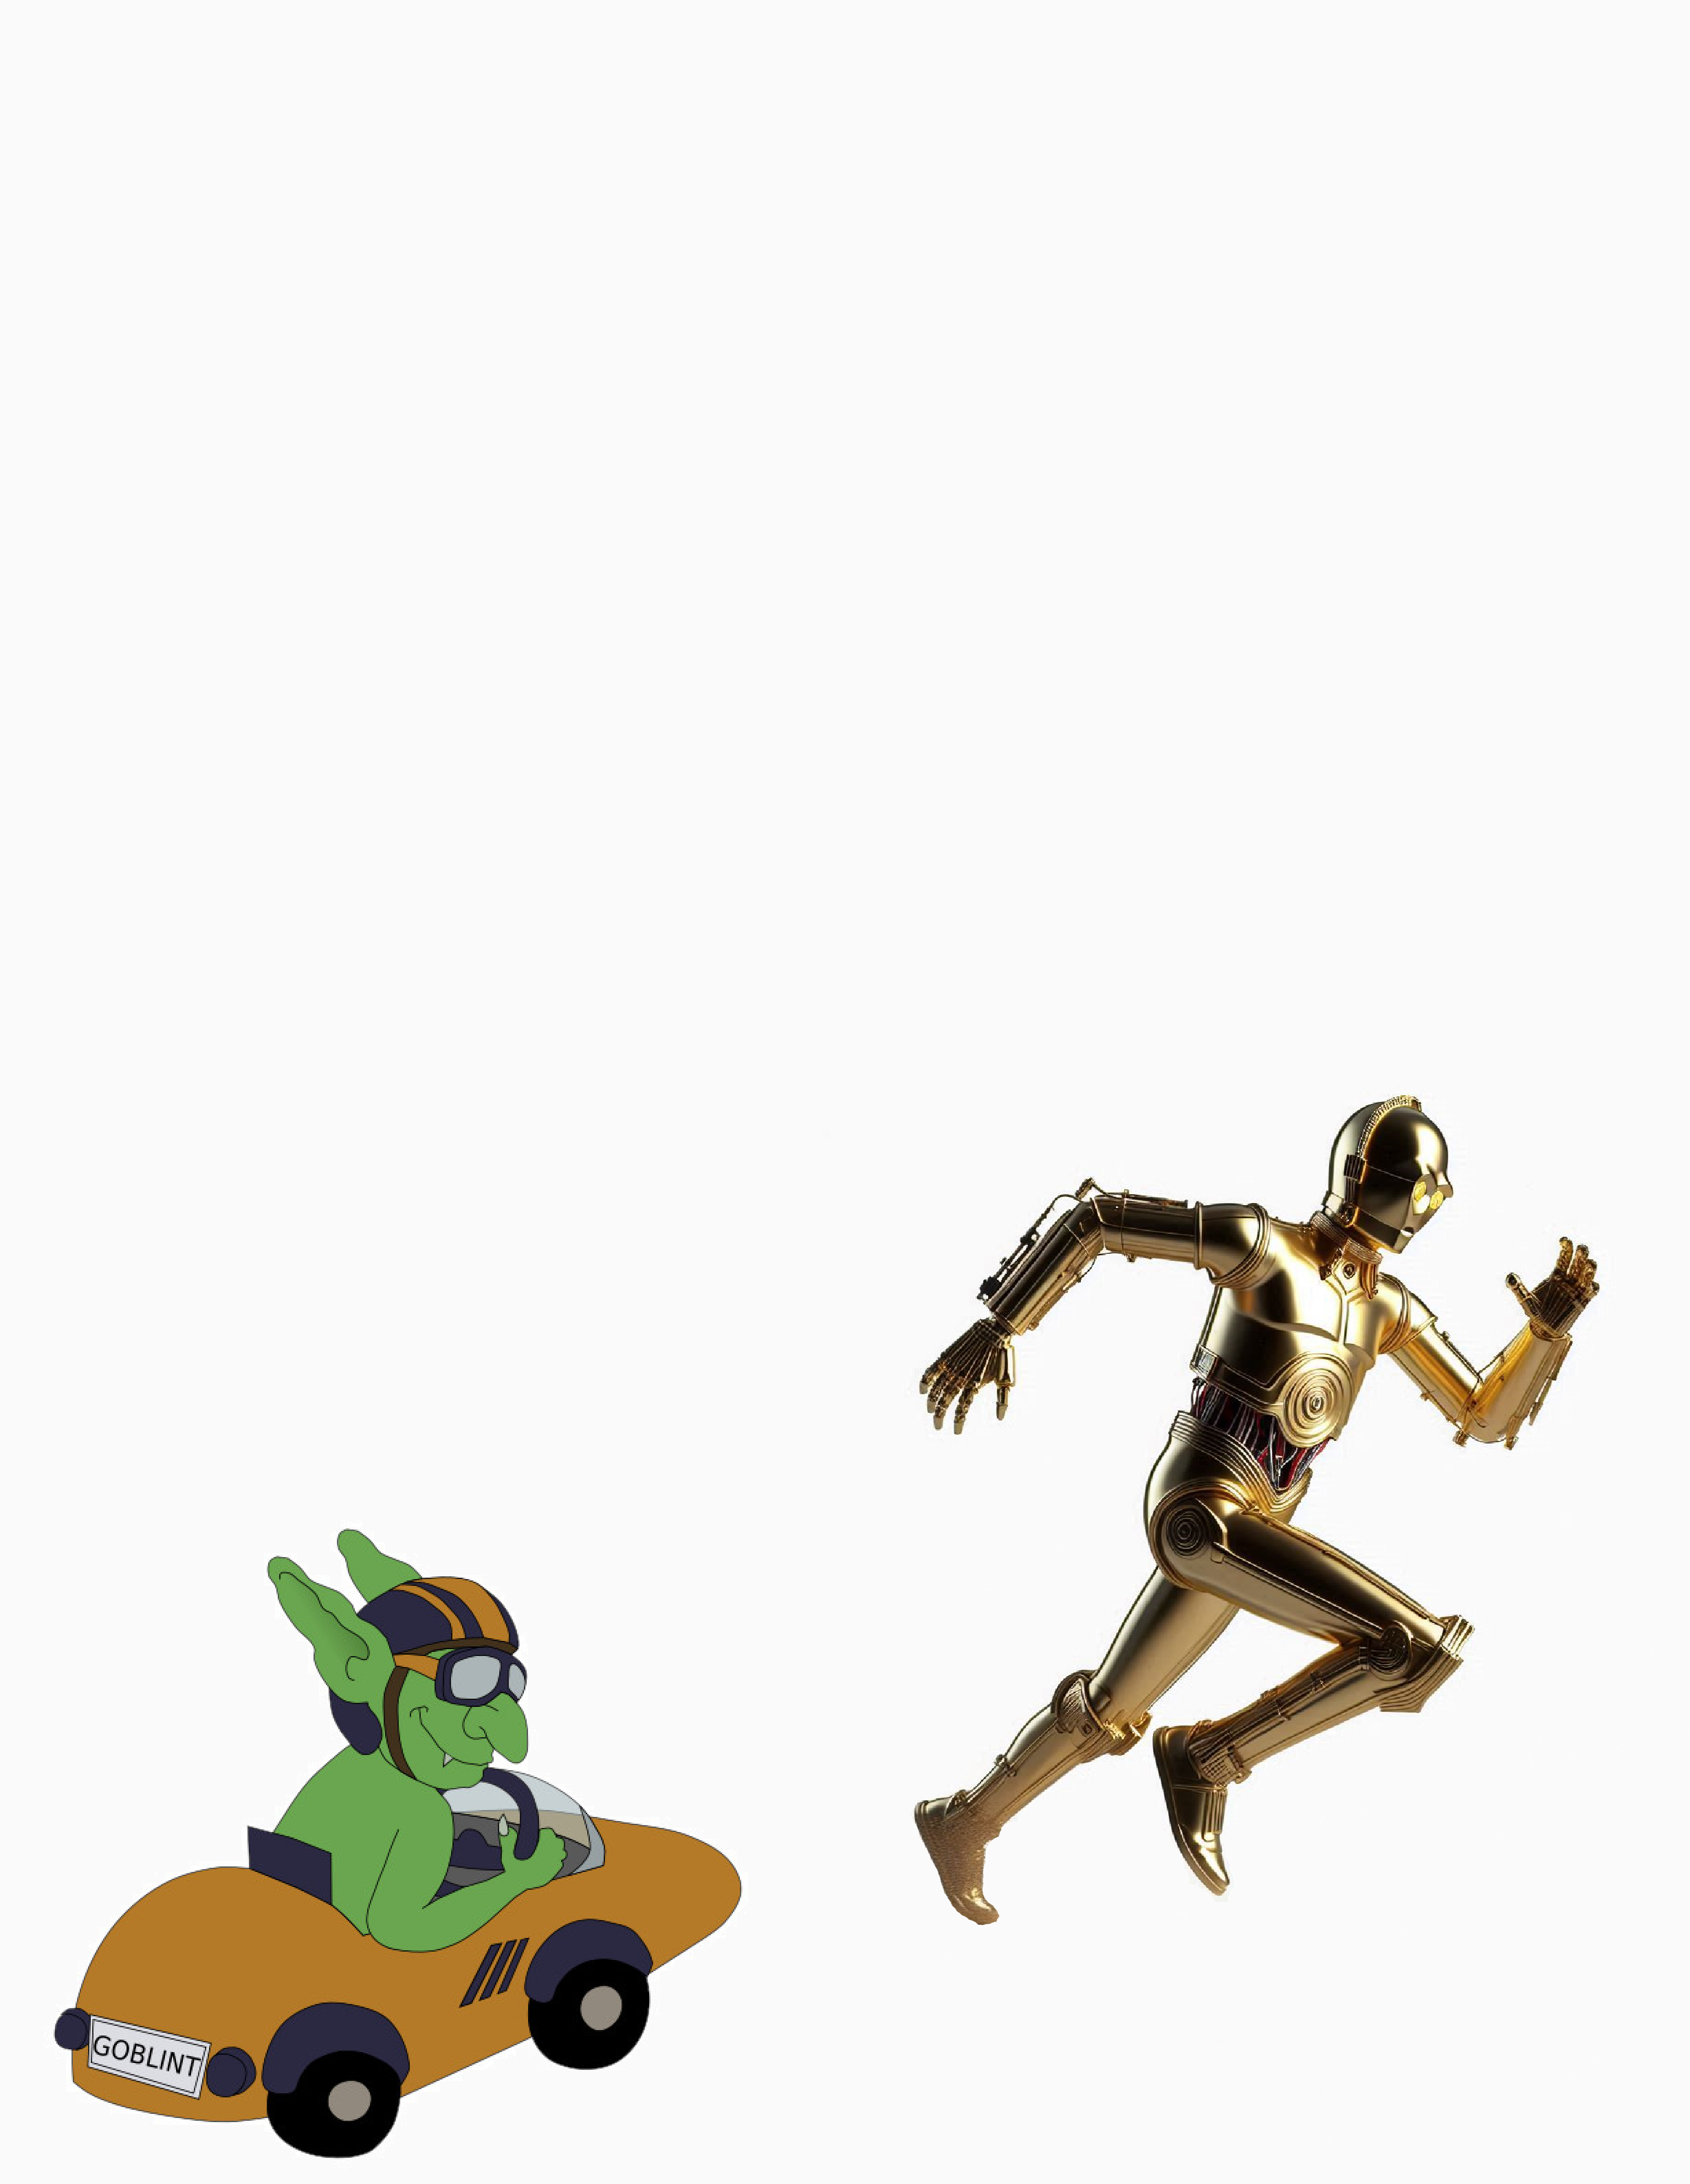
\includegraphics[width=6cm]{images/Goblint car with C-3PO-presentation2.png}}
\institute{
\includegraphics[width=1.5cm]{images/tum-black.pdf}}

\begin{document}

\maketitle


\begin{frame}{\cpo{}: A Weakly-Relational Pointer Analysis for Goblint}


        \textbf{\cpo{}}: C analysis based on 2-Pointer Logic, introduced by Helmut Seidl,
        Julian Erhard,
        Michael Schwarz,
        Sarah Tilscher~\cite{2pointer}


    \[
        (\&x = \&y) \land (x \neq *(1 + A))
    \]

\end{frame}


\begin{frame}[fragile,containsverbatim]{Example}


        \begin{minted}{C}
if(x != 64 + start){
    error();
} else if (*(y+1) == x) {
    success();
}
\end{minted}

\end{frame}

\frame{\tableofcontents}

\section{Abstract Domain}


\begin{frame}{Terms considered by 2-Pointer Logic}
    \begin{itemize}
        \item Atoms: auxiliaries $A$ and address constants $\&x$
              \pause
        \item Terms: atoms + address arithmetic + dereferencing
        \[
            t\,{::=}\,A \mid \&x \mid *(z+t)
        \]
        \pause
        \item $x$ abbreviation for $*(0 + \&x)$ and $*t$ for $*(0+t)$

    \end{itemize}
\end{frame}

\begin{frame}{Propositions considered by 2-Pointer Logic}
    \begin{itemize}
        \item Propositions:
\begin{itemize}
    \item Quantitative equalities
          \[
              t_1=z+t_2
          \]
          \pause
    \item Quantitative disequalities
          \[
              t_1\neq z+t_2
          \]
          \pause

    \item Block disequalities
          \[
              bl(t_1) \neq bl(t_2)
          \]
\end{itemize}
\item Partial order: semantic implication:
              \[
                  \Psi \rightarrow \Psi' \quad\Rightarrow\quad  \Psi \leq \Psi'
              \]
    \end{itemize}
\end{frame}

\begin{frame}{Quantitative Finite Automaton (QFA)}
    \[
        \T=\{ \&x, x, A, \&y\}
    \]
    \[
        (\&x = \&y) \land (x = 1 + A)
    \]
    \centering
    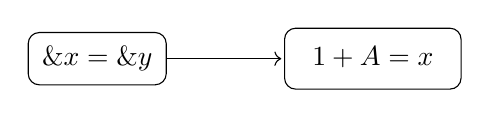
\begin{tikzpicture}[shorten >=1pt, node distance=5cm, on grid, auto, state/.style={rectangle, rounded corners, draw, inner sep=5pt, align=center}]

        \node[state] (y) {$\&x =\&y$};

        \node[state, right=3.5cm of y] (AB) {$\begin{array}{c}
                    1 + A = x
                \end{array}$};

        \path[->]
        (y) edge[] (AB);


    \end{tikzpicture}
\end{frame}

\begin{frame}{QFA: Insert Terms}
    \[
        \T=\{\&x, x, A, \&y, \textcolor{TUMAccentOrange}{y}\}
    \]
    \[
        (\&x = \&y) \land (x = 1 + A)
    \]
    \centering
    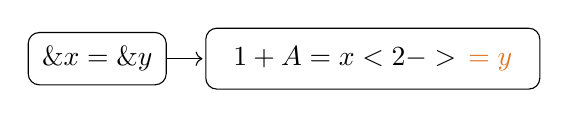
\begin{tikzpicture}[shorten >=1pt, node distance=5cm, on grid, auto, state/.style={rectangle, rounded corners, draw, inner sep=5pt, align=center}]

        \node[state] (y) {$\&x =\&y$};

        \node[state, right=3.5cm of y] (AB) {$\begin{array}{c}
                    1 + A = x
                    \only<2->{\textcolor{TUMAccentOrange}{\,= y}}
                \end{array}$};


        \path[->]
        (y) edge[] (AB);


    \end{tikzpicture}


\end{frame}

\begin{frame}{QFA: Remove Terms}
    \[
        \T=\{\text{\textcolor{TUMAccentOrange}{\sout{$\&x, x, $}}}A, \&y, y\}
    \]
    \[
        (x = 1 + A) \land (\&x = \&y)
    \]
    \centering
    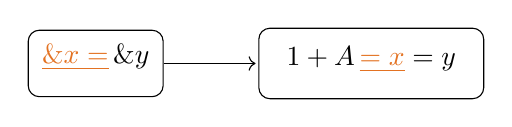
\begin{tikzpicture}[shorten >=1pt, node distance=5cm, on grid, auto, state/.style={rectangle, rounded corners, draw, inner sep=5pt, align=center}]

        \node[state] (y) {$\text{\textcolor{TUMAccentOrange}{\sout{\&x=}}} \,\&y$};

        \node[state, right=3.5cm of y] (AB) {$\begin{array}{c}
                    1 + A \, \text{\textcolor{TUMAccentOrange}{\sout{= x}}}
                    = y
                \end{array}$};


        \path[->]
        (y) edge[] (AB);


    \end{tikzpicture}

\end{frame}

\begin{frame}[fragile,containsverbatim]{Quantitative Disequalities}
    \begin{itemize}
        \item Deriving from block disequalities:
              \[
                  bl(t_1) \neq bl(t_2) \quad\Rightarrow\quad  t_1\neq z+ t_2 \quad\quad \text{for each $z \in \Z$}
              \]
              \pause
        \item Deriving from equalities:
              \[
                  t_1 = z + t_2  \quad\Rightarrow\quad t_1\neq z' + t_2 \quad\quad \text{for each $z' \neq z$}
              \]
              \pause
        \item Deriving from guards:

        \begin{minipage}{0.4\textwidth}
\begin{minted}{C}
        if(*x != 4 + y){...}
\end{minted}
\end{minipage}
\begin{minipage}{0.45\textwidth}
\[
    \quad\Rightarrow\quad *x\neq 4 + y
\]
\end{minipage}

              \pause
        \item Deriving from other disequalities:
              \[ *(z_1 + t_1) \neq *(z_2 + t_2) \quad\Rightarrow\quad z_1 + t_1 \neq z_2 + t_2
              \]
    \end{itemize}
\end{frame}

\section{Meet}
\begin{frame}{Meet}
    \begin{itemize}

        \item Greatest lower bound of $\Psi$ and $\Psi'$ $\rightarrow$ $\Psi \land \Psi'$
              \pause
        \item Add equalities to QFA
              \pause
        \item Add block/quantitative disequalities
              \pause
        \item Closure of disequalities
    \end{itemize}
\end{frame}


\section{Join}
\begin{frame}{Join}
    \begin{itemize}
        \item Least upper bound of $\Psi$ and $\Psi'$ $\rightarrow$ $\Psi \lor \Psi'$
              \pause
        \item Not always representable as a finite conjunction~\cite{join}

    \end{itemize}
\end{frame}

\begin{frame}{Join of two QFAs $M_1 \join M_2$:}
    \begin{itemize}
        \item Add terms to $M_1$ and $M_2$ to bring them to the same set of terms
        \pause
        \item Group terms by their
              \begin{itemize}
                  \item Equivalence class of $M_1$
                  \item Equivalence class of $M_2$
                  \item Same distance in $M_1$ and $M_2$
              \end{itemize}
              \pause
        \item[$\rightarrow$] product automaton with offset
    \end{itemize}
\end{frame}

\begin{frame}{Join: Group by Offset}
    \[
        \T = \{
        A,B,C
        \}
    \]
    \begin{minipage}{0.45\textwidth}
        \centering
        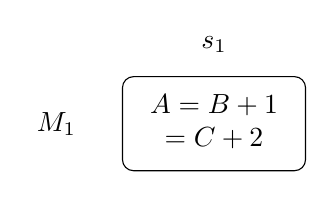
\begin{tikzpicture}[shorten >=1pt, node distance=3cm, on grid, auto, state/.style={rectangle, rounded corners, draw, inner sep=5pt, align=center}]

            \node[state] (Q1) {$\begin{array}{c}A = B+1\\ = C + 2\end{array}$};
            \node[above=1cm of Q1] (s1) {$s_1$};
            \node[left=2cm of Q1] (m1) {$\boldsymbol{M_1}$};



        \end{tikzpicture}

        \vspace*{1cm}

        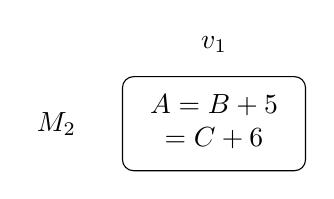
\begin{tikzpicture}[shorten >=1pt, node distance=3cm, on grid, auto, state/.style={rectangle, rounded corners, draw, inner sep=5pt, align=center}]

            \node[state] (Q1) {$\begin{array}{c}A = B+5\\ = C + 6\end{array}$};
            \node[above=1cm of Q1] (s1) {$v_1$};
            \node[left=2cm of Q1] (m1) {$\boldsymbol{M_2}$};

        \end{tikzpicture}
    \end{minipage}
    \begin{tikzpicture}[overlay]
        \draw[->, thick] (0, 0) -- (1, 0);
    \end{tikzpicture}
    \hfill%
    \begin{minipage}{0.4\textwidth}

        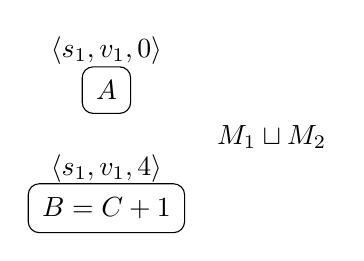
\begin{tikzpicture}[shorten >=1pt, node distance=1.5cm, on grid, auto, state/.style={rectangle, rounded corners, draw, inner sep=5pt, align=center, minimum size=0.5cm}]

            \node[state] (Q1) {$A$};
            \node[state, below= 1.5cm of Q1] (Q2) {$B = C + 1$};
            \node[below right=0.6cm and 2.1cm of Q1] (m1) {$\boldsymbol{M_1 \join M_2}$};

            \node[above=0.5cm of Q1] (s1) {$\angl{s_1,v_1, 0}$};
            \node[above=0.5cm of Q2] (s1) {$\angl{s_1,v_1, 4}$};

        \end{tikzpicture}
    \end{minipage}
\end{frame}

\section{Widening and Narrowing}
\begin{frame}{Widening and Narrowing}

    \begin{itemize}
        \item Limit the terms of the result to the set of terms of the first element
    \end{itemize}
    %\[\Psi_1 \widen \Psi_2 = \restr{(\Psi_1 \join \Psi_2)}{\T_1}.\]
    %\[\Psi_1 \narrow \Psi_2 = \restr{(\Psi_1 \meet \Psi_2)}{\T_1}.\]
    \begin{itemize}
        \pause
        \item Limit the possible offsets
              appearing in disequalities
    \end{itemize}

\end{frame}

\section{Assignment}

\begin{frame}{Assignment to an Unknown Expression}
    \[
        t_1\,{:=}\,?
    \]
    \begin{itemize}
        \item Forget all terms that may be modified $\rightarrow$ terms with the same address as $t_1$
              \pause
        \item If $t_1 = A$ or $t_1 = \&x$: remove terms that have $t_1$ as subterm
              \pause
        \item If $t_1 = *(z + t)$: keep only terms $*(z' + v)$ where
              \begin{itemize}
                  \item can infer $z + t \neq z' + v$ %or $bl(t) \neq bl(v)$
                        % \item $t = z_1 + v$ and $z_1 \neq (z' - z)$ %and they do not overlap
                  \item use non-relational analysis: possible values of $z + t$ and $z' + v$ do not intersect
              \end{itemize}
    \end{itemize}
\end{frame}

\begin{frame}{Assignment to a Term with an Offset}
    \[
        t_1\,{:=}\,z + t
    \]
    \begin{itemize}
        \item Fresh auxiliary $A$
        \item Add equality $A = z + t$
        \item Remove terms modified by an assignment to $t_1$
        \item Add equality $t_1 = A$
        \item Remove $A$
    \end{itemize}
\end{frame}

\begin{frame}{Dynamic Memory Allocation}
    \[
        t_1\,{:=}\,\malloc
    \]
    \begin{itemize}
        \pause
        \item Remove terms modified by an assignment to $t_1$
              \pause
        \item For each $t \in \T$, add:
              \[
                  bl(t) \neq bl(t_1)
              \]
    \end{itemize}
\end{frame}

\section{Evaluation}

\begin{frame}{Precision Test Suite}
    \begin{itemize}
        \item GNU Core Utilities (Coreutils), automatically annotated invariants by \cpo\
              \pause
        \item Compared three different \goblint\ analyses:
              \begin{itemize}
                  \item \base{}: basic \goblint\ analysis, including a non-relational pointer analysis
                  \item \vareq{}: tracks must-equalities between general expressions
                  \item \cpo\
              \end{itemize}
    \end{itemize}
\end{frame}

\begin{frame}{Coreutils Test Results}
    \centering

    \begin{tikzpicture}
        \begin{axis}[
                ybar,
                symbolic x coords={\base, \vareq, \cpo},
                xtick=data,
                ymin=0, ymax=19488,
                bar width=1cm,
                ylabel={Number of Proven Assertions},
                xlabel={Analyses},
                scaled y ticks=false,
                %ytick={0,5000,10000,15000},
                %yticklabels={0,{5,000},{10,000},{15,000}},
                nodes near coords,
                nodes near coords align={vertical},
            ]
            \addplot coordinates {(\base, 4636) (\vareq, 8188) (\cpo, 19488)};
        \end{axis}
    \end{tikzpicture}

\end{frame}


\begin{frame}{Performance: SV-Comp Results}
    \centering

    \begin{tikzpicture}
        % Load the picture
        \node[anchor=south west,inner sep=0] (image) at (0,0) {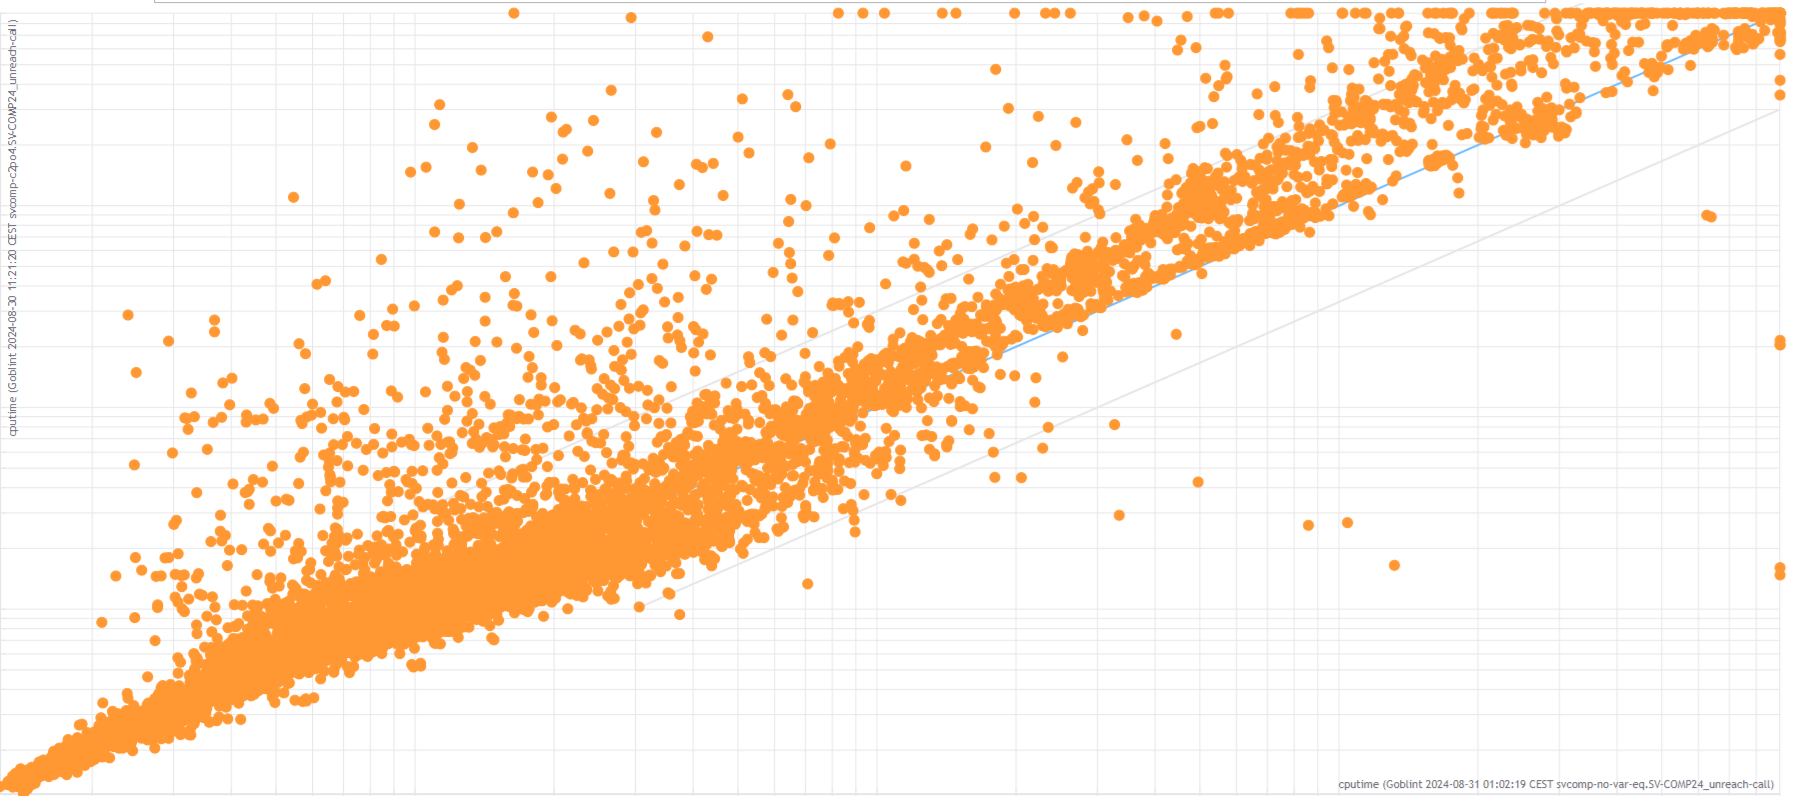
\includegraphics[width=10cm]{images/base-vs-cpo4-cropped.png}};

        % Overlaying axes with logarithmic scales
        \begin{axis}[
                width=11.57cm, % Match the width of the image
                height=6cm, % Adjust as needed
                at={(image.south west)}, % Position the axis on the image
                anchor=south west, % Anchors the axis to the southwest corner of the image
                axis on top, % Ensure the axes are drawn on top of the image
                xmin=1, xmax=900, % Define the x-axis limits
                ymin=1, ymax=900, % Define the y-axis limits
                xmode=log, % Logarithmic x-axis
                ymode=log, % Logarithmic y-axis
                xlabel={\base}, % X-axis label
                ylabel={\cpo}, % Y-axis label
                xtick={1,10,100,900}, % X-axis ticks in logarithmic scale
                ytick={1,10,100,900}, % Y-axis ticks in logarithmic scale
                xticklabels={0, 10, 100, 900}, % Custom x-axis labels
                yticklabels={0, 10, 100, 900}, % Custom y-axis labels
                grid=none, % Show the grid for better visualization
                minor tick num=9, % Number of minor ticks between major ticks
            ]

            \addplot[domain=1:900, samples=100, thick, TUMBlue!60] {x};

        \addplot[domain=1:900, samples=100, TUMBlue!60] {2.35*x};

        \addplot[domain=1:900, samples=100, TUMBlue!60] {0.43*x};

        \end{axis}

    \end{tikzpicture}
\end{frame}

\begin{frame}{Related Work}
    \begin{itemize}
        \item non-relational pointer analysis
        \[
        p \mapsto \{ \&malloc_1, \&y \}
        \]
        \begin{itemize}
            \item fast flow- and context-insensitive \cite{Steensgaard,Andersen}
            \item flow- and context-sensitive (Mopsa~\cite{mopsa},
            Frama-C~\cite{framac}, \goblint~\cite{goblint})
        \end{itemize}
        \pause
        \item very precise shape analysis, e.g., separation logic~\cite{separationlogic,rivalpapers}
        \[
             \{(x + 4 \mapsto 4)\ast ((x\mapsto 42){-\!\!*}P)\}
        \]

    \end{itemize}
\end{frame}

\section{Conclusion}

\begin{frame}{Conclusion}
    \begin{itemize}
        \item \cpo\ can infer equalities and disequalities between two pointer expressions % that were out of reach for other goblint analyses
        \pause
        \item Implemented meet and (approximation of) join
        \pause
        \item Widening and narrowing for termination
        \pause
        \item Increase precision by cooperating with non-relational analysis
        \pause
        \item Future work: track null pointers/undefined pointers
    \end{itemize}
    %was haben wir gelernt, ist sie geeignet, was sind die vorteile
    %man kann auch unsere analyse benutzen um zu wissen, ob sachen bei einem assignment überschrieben werden, so wie wir die non-relational pointer analyse benutzen
\end{frame}

\begin{frame}
    \centering
\huge
       \textbf{Thank you for listening}


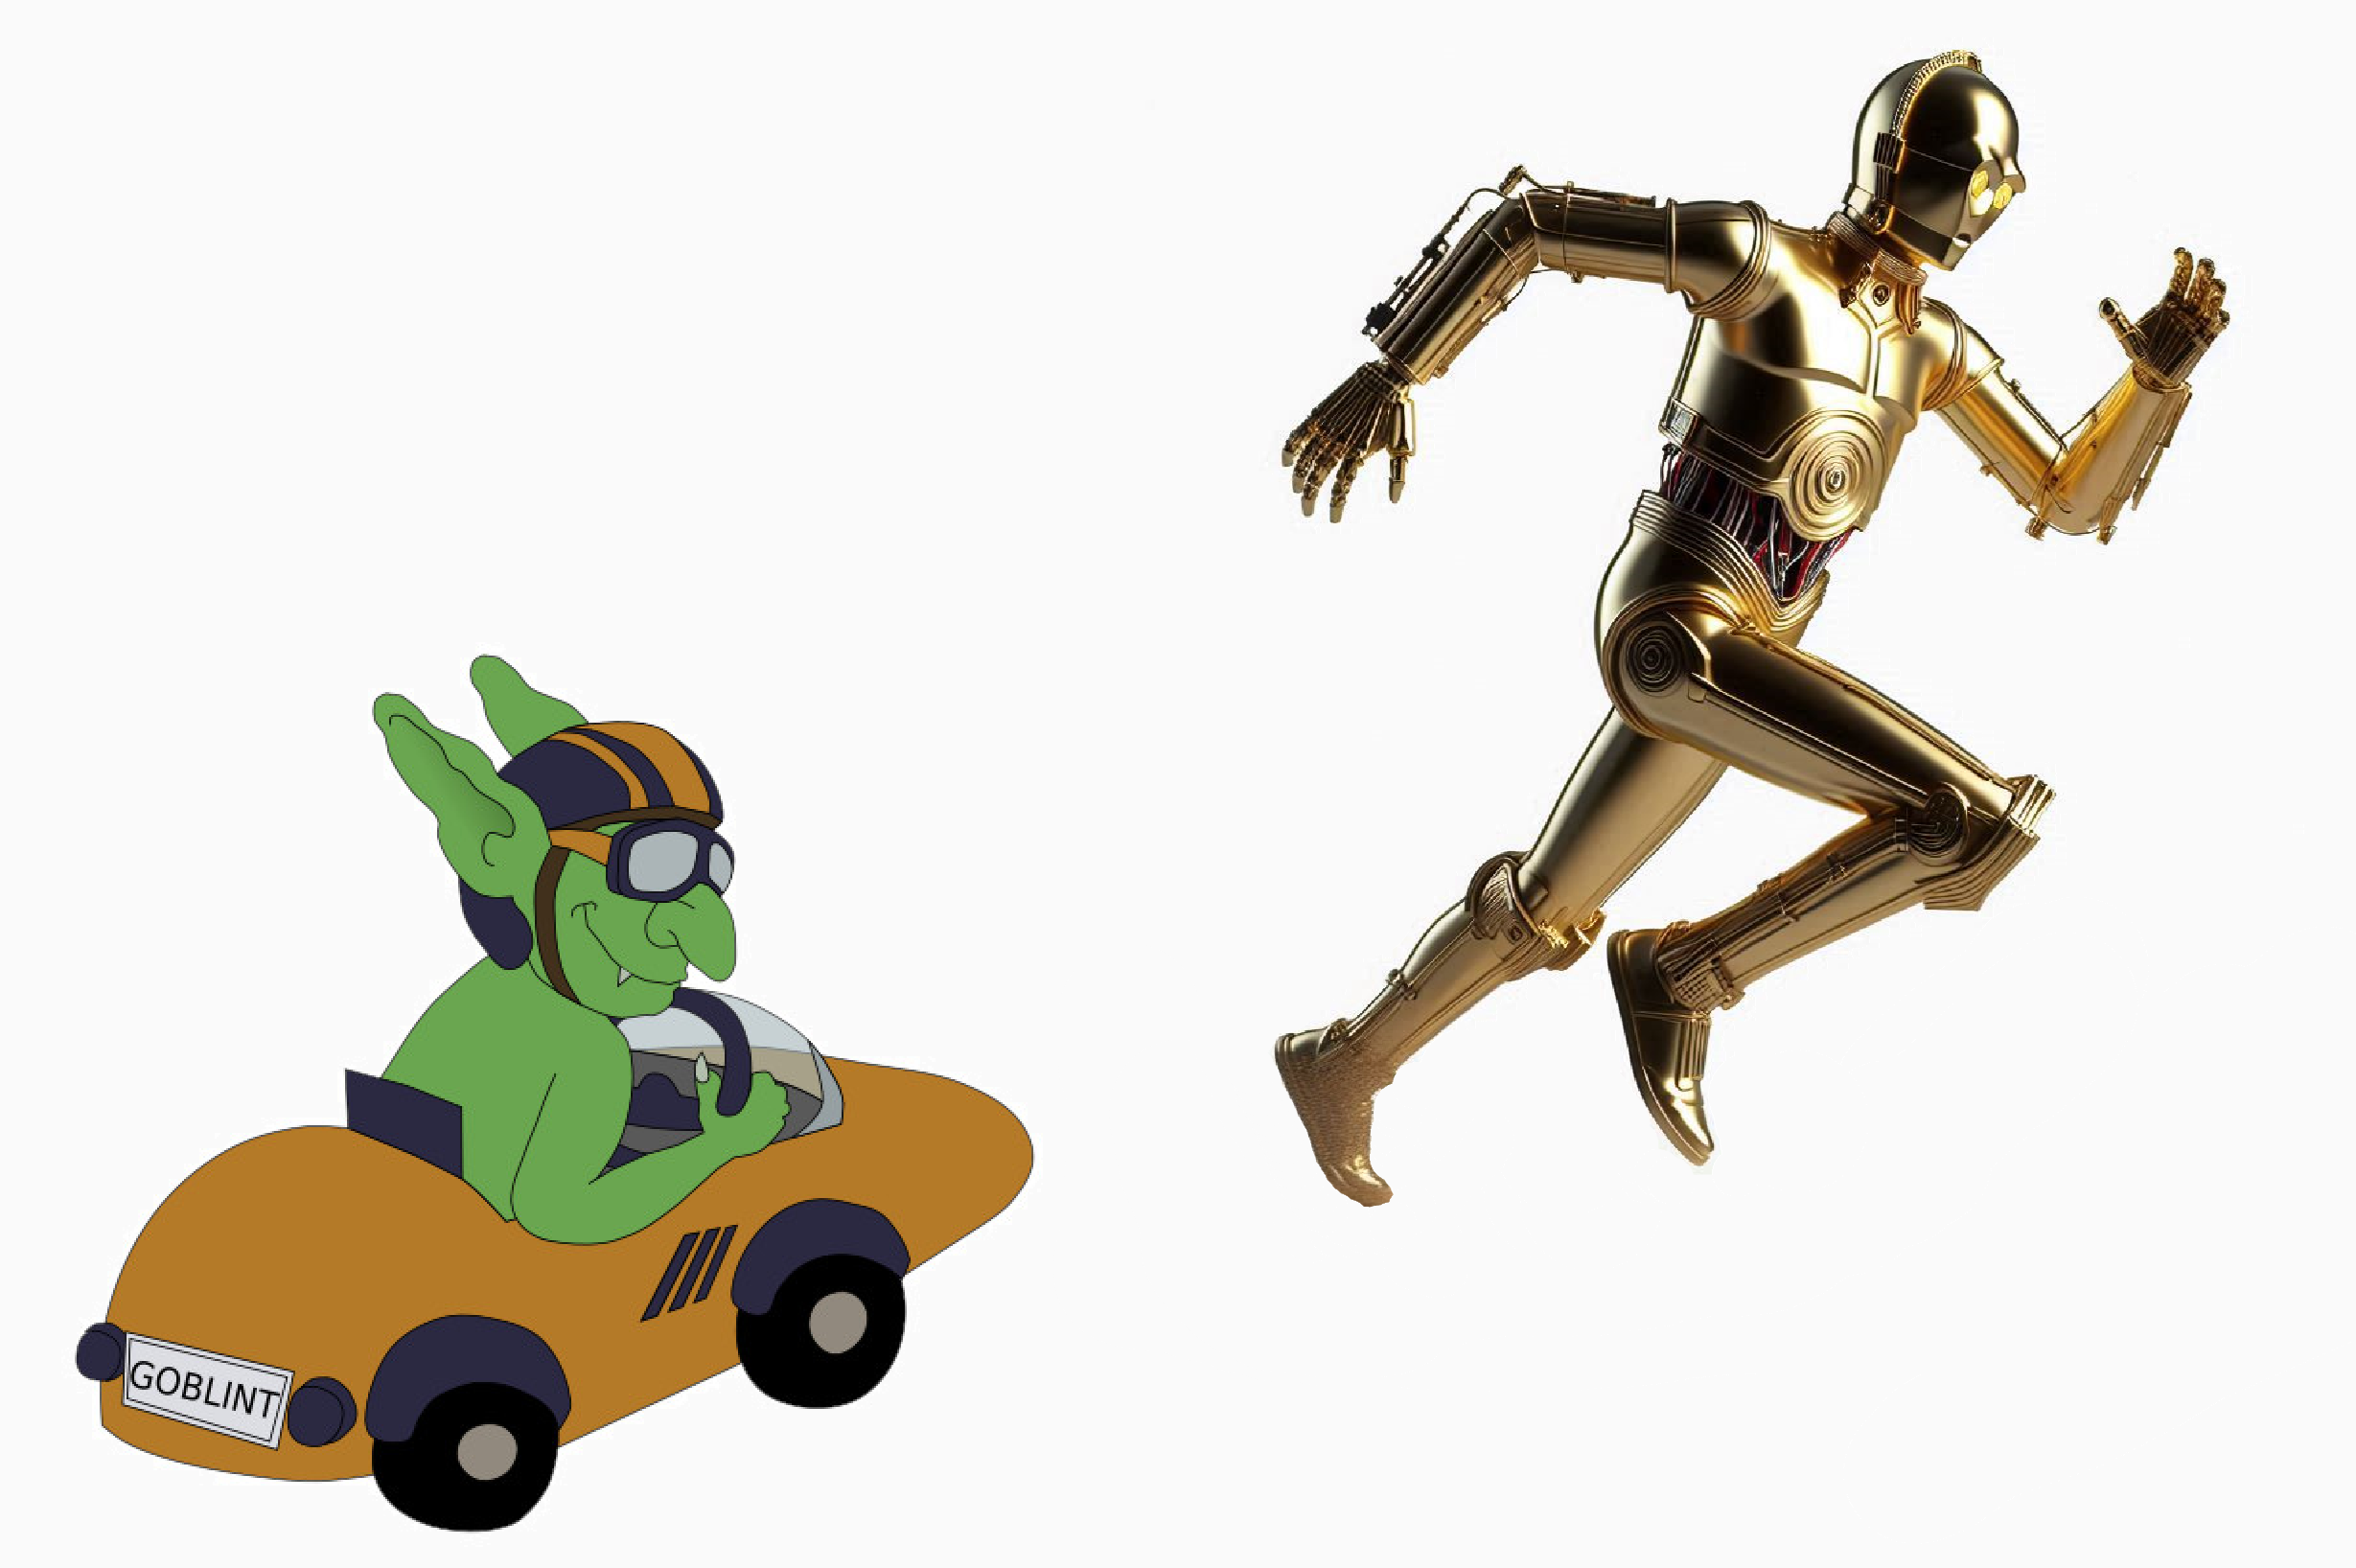
\includegraphics[width=6cm]{images/Goblint car with C-3PO-presentation3.png}
\end{frame}

\appendix

 \begin{frame}[allowframebreaks]
     \frametitle{References}
     \bibliographystyle{amsalpha}
     \bibliography{main.bib}
 \end{frame}


\begin{frame}{Two-dimensional Memory Model}
    \begin{itemize}
        \item In C: pointer arithmetic is not allowed to go outside the current memory object
        \item Address: (blockID, offset)
        \item $bl(a,b) = a$

    \end{itemize}
    \begin{tikzpicture}

        \def\blockheight{0.8}
        \def\startx{0}

        \draw (\startx, 0) rectangle (\startx + 3, -\blockheight);
        \node[anchor=west] at (\startx, -0.5*\blockheight) {int x};
        \draw (\startx, -\blockheight) rectangle (\startx + 5, -2*\blockheight);
        \node[anchor=west] at (\startx, -1.5*\blockheight) {struct a};
        \draw (\startx, -2*\blockheight) rectangle (\startx + 7, -3*\blockheight);
        \node[anchor=west] at (\startx, -2.5*\blockheight) {int a[5]};
        \draw (\startx, -3*\blockheight) rectangle (\startx + 9, -4*\blockheight);
        \node[anchor=west] at (\startx, -3.5*\blockheight) {malloc\#001};

        \draw[->] (\startx,  -4*\blockheight) -- (\startx + 10, -4*\blockheight) node[anchor=north] {Offset};
        \draw[->] (\startx,  -4*\blockheight) -- (\startx, \blockheight) node[anchor=south, rotate=90] {BlockID};

        \node[anchor=east] at (\startx, -1*\blockheight) {3};
        \node[anchor=east] at (\startx, -2*\blockheight) {2};
        \node[anchor=east] at (\startx, -3*\blockheight) {1};
        \node[anchor=east] at (\startx, -4*\blockheight) {0};

        \foreach \x in {0, 2, 4, 6, 8} {
                \draw (\startx + \x, -4*\blockheight) -- (\startx + \x, -4*\blockheight);
                \node[anchor=north] at (\startx + \x, -4*\blockheight) {\x};
            }

    \end{tikzpicture}
\end{frame}

\begin{frame}{Representation of structs and arrays}
    \begin{itemize}
        \item $a[1]\equiv *(a+1)$
        \item $a[i][j] \equiv (a + (i \cdot m + j) \cdot 32) \quad \text{for \texttt{int a[n][m]}}$
        \item struct $s$: $s.f \equiv *(\&s + 32)$
    \end{itemize}
\end{frame}



\begin{frame}{When is the Meet Unsatisfiable?}
    \begin{itemize}

        \item $t_1 = z + t_2$, and $t_1 = z' + t_2$, but $z\neq z'$

        \item $t_1 = z + t_2$, and $t_1 \neq z + t_2$

        \item $t_1 = z + t_2$, and $bl(t_1) \neq bl(t_2)$


    \end{itemize}
\end{frame}


\begin{frame}{Not Finitely Representable Join}
    \begin{itemize}
        \item It is not always possible to calculate the join
    \end{itemize}

    \[
        (A = V)
    \]

    \[
        (*A = A)\land (*V=V) \land (*(1 + A) = *(1 + V))
    \]
    \begin{itemize}
        \item Join:
    \end{itemize}
    \[
        *(1+*^n A) = *(1 + *^n V)\quad\quad\text{ for each $n \geq 0$}
    \]
\end{frame}

% \begin{frame}{Interprocedural}
%     enter:
%     \begin{itemize}
%         \item Remove local variables of caller.
%         \item Add shadow variable $p'$ for each parameter $p$ and the equality $p = p'$.
%     \end{itemize}
%     combine:
%     \begin{itemize}
%         \item Remove tainted variables from caller state.
%         \item Meet caller and callee state.
%         \item Add equality $p' = e$ for each parameter $p$ called with the expression $e$.
%         \item Assign return value to variable if necessary.
%         \item Remove local variables of callee and shadow variables.
%     \end{itemize}
% \end{frame}

\begin{frame}{Not Finitely Representable Join}
    \begin{minipage}{0.45\textwidth}
        \centering
        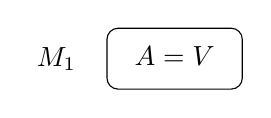
\begin{tikzpicture}[shorten >=1pt, node distance=3cm, on grid, auto, state/.style={rectangle, rounded corners, draw, inner sep=5pt, align=center}]

            \node[state] (Q1) {$\begin{array}{c}
                        A=V
                    \end{array}$};
            \node [left=1.5cm of Q1] {$\boldsymbol{M_1}$};
        \end{tikzpicture}

    \end{minipage}
    \begin{minipage}{0.45\textwidth}

        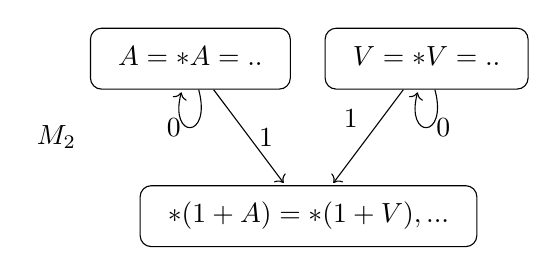
\begin{tikzpicture}[shorten >=1pt, node distance=3cm, on grid, auto, state/.style={rectangle, rounded corners, draw, inner sep=5pt, align=center}]

            \node[state] (Q1) {$\begin{array}{c}
                        A=*A=..
                    \end{array}$};

            \node[state, right=3cm of Q1] (Q2) {$\begin{array}{c}
                        V=*V=..
                    \end{array}$};

            \node[state, below right=2cm and 1.5cm of Q1] (Q3) {$\begin{array}{c}
                        *(1+A)= *(1 + V),...
                    \end{array}$};

            \path[->]
            (Q1) edge[loop below] node[left] {$0$} (Q1)
            (Q2) edge[loop below] node[right] {$0$} (Q2)
            (Q1) edge[] node[right] {$1$} (Q3)
            (Q2) edge[] node[above left] {$1$} (Q3);

            \node [below left=1cm and 1.7cm of Q1] {$\boldsymbol{M_2}$};

        \end{tikzpicture}
    \end{minipage}

\end{frame}



\begin{frame}{Join: Product Automaton}
    \[
        \T = \{
        \&x,x,*x, {*}{*}x
        \}
    \]
    \begin{minipage}{0.4\textwidth}
        \centering
        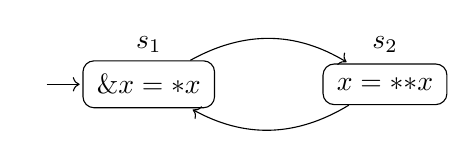
\begin{tikzpicture}[shorten >=1pt, node distance=3cm, on grid, auto, state/.style={rectangle, rounded corners, draw, inner sep=5pt, align=center}]

            \node[state, initial, initial text={}] (Q1) {$\&x= *x$};
            \node[state, right=of Q1] (Q2) {$x= {*}{*}x$};
            \node[above=0.5cm of Q1] (s1) {$s_1$};
            \node[above=0.5cm of Q2] (s2) {$s_2$};


            \path[->]
            (Q1) edge[bend left, above] (Q2)
            (Q2) edge[bend left, below] (Q1);

        \end{tikzpicture}

        \vspace*{1cm}

        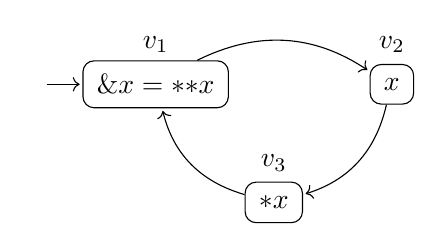
\begin{tikzpicture}[shorten >=1pt, node distance=3cm, on grid, auto, state/.style={rectangle, rounded corners, draw, inner sep=5pt, align=center}]

            \node[state, initial, initial text={}] (Q1) {$\&x= {*}{*}x$};
            \node[state, right=of Q1] (Q2) {$x$};
            \node[state, below right=1.5cm and 1.5cm of Q1] (Q3) {$*x$};
            \node[above=0.5cm of Q1] (s1) {$v_1$};
            \node[above=0.5cm of Q2] (s2) {$v_2$};
            \node[above=0.5cm of Q3] (s3) {$v_3$};

            \path[->]
            (Q1) edge[bend left] (Q2)
            (Q2) edge[bend left] (Q3)
            (Q3) edge[bend left] (Q1);

        \end{tikzpicture}
    \end{minipage}
    \begin{tikzpicture}[overlay]
        \draw[->, thick] (0, 0) -- (1, 0);
    \end{tikzpicture}
    \hfill%
    \begin{minipage}{0.49\textwidth}

        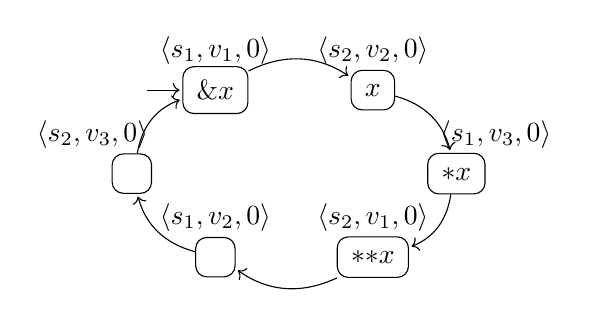
\begin{tikzpicture}[shorten >=1pt, node distance=1.5cm, on grid, auto, state/.style={rectangle, rounded corners, draw, inner sep=5pt, align=center, minimum size=0.5cm}]

            \node[state, initial, initial text=] (Q1) {$\&x$};
            \node[state, right=2cm of Q1] (Q2) {$x$};
            \node[state, below right=of Q2] (Q3) {$*x$};
            \node[state, below left=of Q3] (Q4) {${*}{*}x$};
            \node[state, left=2 cmof Q4] (Q5) {};
            \node[state, above left=of Q5] (Q6) {};
            \node[above=0.5cm of Q1] (s1) {$\angl{s_1,v_1,0}$};
            \node[above=0.5cm of Q2] (s2) {$\angl{s_2,v_2,0}$};
            \node[above right=0.5cm and 0.5cm of Q3] (s3) {$\angl{s_1,v_3,0}$};
            \node[above=0.5cm of Q4] (s4) {$\angl{s_2,v_1,0}$};
            \node[above=0.5cm of Q5] (s5) {$\angl{s_1,v_2,0}$};
            \node[above left=0.5cm and 0.5cm of Q6] (s6) {$\angl{s_2,v_3,0}$};



            \path[->]
            (Q1) edge[bend left] (Q2)
            (Q2) edge[bend left] (Q3)
            (Q3) edge[bend left] (Q4)
            (Q4) edge[bend left] (Q5)
            (Q5) edge[bend left] (Q6)
            (Q6) edge[bend left] (Q1)
            ;

        \end{tikzpicture}
    \end{minipage}
\end{frame}


\begin{frame}{Join: Add Terms to Empty Equivalence Classes}
    %overapproximation

    \begin{itemize}
        \item Add a term for each empty state in the automaton
    \end{itemize}
    \[
        \T = \{
        \&x,x,*x, {*}{*}x,\textcolor{TUMAccentOrange}{{*}{*}{*}x,{*}{*}{*}{*}x}
        \}
    \]

    \centering
    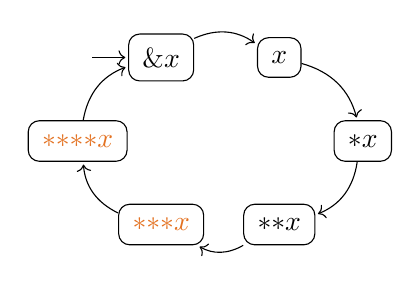
\begin{tikzpicture}[shorten >=1pt, node distance=1.5cm, on grid, auto, state/.style={rectangle, rounded corners, draw, inner sep=5pt, align=center, minimum size=0.5cm}]

        \node[state, initial, initial text=] (Q1) {$\&x$};
        \node[state, right= 1.5cm of Q1] (Q2) {$x$};
        \node[state, below right=of Q2] (Q3) {$*x$};
        \node[state, below left=of Q3] (Q4) {${*}{*}x$};
        \node[state, left=of Q4] (Q5) {$\textcolor{TUMAccentOrange}{{*}{*}{*}x}$};
        \node[state, above left=of Q5] (Q6) {$\textcolor{TUMAccentOrange}{{*}{*}{*}{*}x}$};
        \path[->]
        (Q1) edge[bend left] (Q2)
        (Q2) edge[bend left] (Q3)
        (Q3) edge[bend left] (Q4)
        (Q4) edge[bend left] (Q5)
        (Q5) edge[bend left] (Q6)
        (Q6) edge[bend left] (Q1)
        ;

    \end{tikzpicture}
\end{frame}

\begin{frame}{Infinite ascending/descending chains}
    \begin{itemize}
        \item Infinite strictly ascending chain:
    \end{itemize}
    \[
        \Psi_n \equiv (*^{2^n} \&x = \&x)\hspace{6pt} (n\geq 0).
    \]
    \begin{itemize}
        \item Infinite strictly descending chains:
    \end{itemize}
    \[
        \Phi_n \equiv\bigwedge_{i=1}^n (\&y = *(i+\&x))\qquad(n\geq 0)
    \]
    \[
        \Psi_n \equiv (y\neq n+\&x)\qquad(n\geq 0)
    \]
\end{frame}


% \begin{frame}[fragile,containsverbatim]{Example}
%     %(etwas was goblint noch nicht konnte auch nicht mit var eq
%     %-> running example)
%     \begin{minipage}{0.49\textwidth}

%         \begin{tikzpicture}

%             % Settings
%             \def\blockheight{0.8}
%             \def\blockwidth{3.5}

%             % Memory blocks and addresses
%             \foreach \i/\label in {0/malloc1, 1/free1, 2/malloc2, 3/free2, 4/malloc3, 5/free3, 6/malloc4, 7/free4} {
%                     % Draw memory block
%                     \draw (0, -\i*\blockheight) rectangle (\blockwidth, -\i*\blockheight - \blockheight);
%                     % Label the memory block
%                     \node at (\blockwidth/2, -\i*\blockheight - \blockheight/2) {\label};
%                     % Print address to the right
%                     \node[above right=0.1cm and 0cm] at (\blockwidth, -\i*\blockheight - \blockheight/2) {\texttt{\the\numexpr 4*\i \relax}};
%                 }
%         \end{tikzpicture}
%     \end{minipage}
%     \begin{minipage}{0.49\textwidth}

%         \begin{minted}{C}
% ...
% p = (*malloc)();
% ...
% (*free)(p);
% ...
% \end{minted}
%         \only<2>{\alert{$\rightarrow$ $free = 4 + malloc$?}}
%     \end{minipage}
% \end{frame}



% \begin{frame}{Litmus Test Results}
%     \begin{itemize}
%         \item 29 litmus tests, manually annotated invariants
%     \end{itemize}
%     \centering

%     \begin{tikzpicture}
%         \begin{axis}[
%                 ybar,
%                 symbolic x coords={\base, \vareq, \cpo},
%                 xtick=data,
%                 ymin=0, ymax=109,
%                 bar width=1cm,
%                 ylabel={Number of Proven Assertions},
%                 xlabel={Analyses},
%                 nodes near coords,
%                 nodes near coords align={vertical},
%             ]
%             \addplot coordinates {(\base, 17) (\vareq, 23) (\cpo, 109)};
%         \end{axis}
%     \end{tikzpicture}

% \end{frame}

% \begin{frame}{Performance Experiments}
%     \begin{itemize}
%         \item Compared efficiency of \goblint\ with \cpo\ and without (\base)
%         \item SV-Comp: large set of verification tasks used for software competition

%         \item 95\% have less than 3x slowdown

%         \item Few additional passed tests; some additional timeouts
%     \end{itemize}
% \end{frame}

\begin{frame}{Overlapping values}

    {
        \centering

        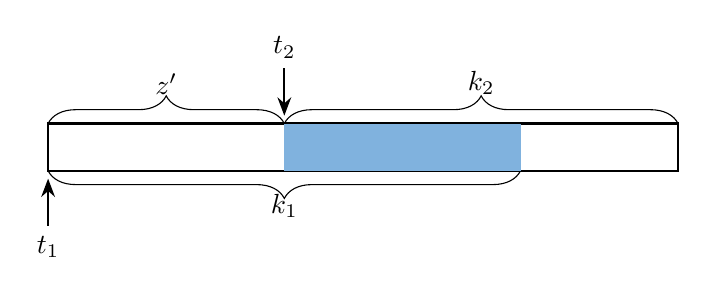
\begin{tikzpicture}[
                memory/.style={draw, thick, minimum height=0.6cm},
                pointer/.style={-Stealth, thick},
                bracket/.style={decorate,decoration={brace, amplitude=10pt, mirror}},
                bracketabove/.style={decorate,decoration={brace, amplitude=10pt}}
            ]

            \draw[memory] (0,0) rectangle (8,0.6);

            \draw[pointer] (3, 1.3) node[above] {$t_2$} -- (3, 0.7);
            \draw[pointer] (0, -0.7) node[below] {$t_1$} -- (0, -0.1);

            \draw[bracketabove] (3, 0.6) -- node[above=7pt] {$k_2$} (8, 0.6);
            \draw[bracketabove] (0, 0.6) -- node[above=7pt] {$z'$} (3, 0.6);
            \draw[bracket] (0, 0) -- node[below=5pt] {$k_1$} (6, 0);

            \draw[dashed] (3, 0) -- (3, 0.6);
            \draw[dashed] (6, 0) -- (6, 0.6);

            \fill[TUMBlue!50] (3,0) rectangle (6,0.6); % overlap

        \end{tikzpicture}
    }
    \begin{itemize}
        \item $t_2 = z' + t_1$.
        \item There is an overlap if $z' < k_1$.
    \end{itemize}

\end{frame}

\end{document}
